\section{Visualization}
\begin{frame}[c]{Visualizing Global Point Cloud Features}
    \Large
    % \begin{itemize}
    %     \item Picture of Architectural overview
    %     \item contributing to global feature: critical points
    %     \item visualizisations, extend to upper bound shape
    % \end{itemize}
    \centering
    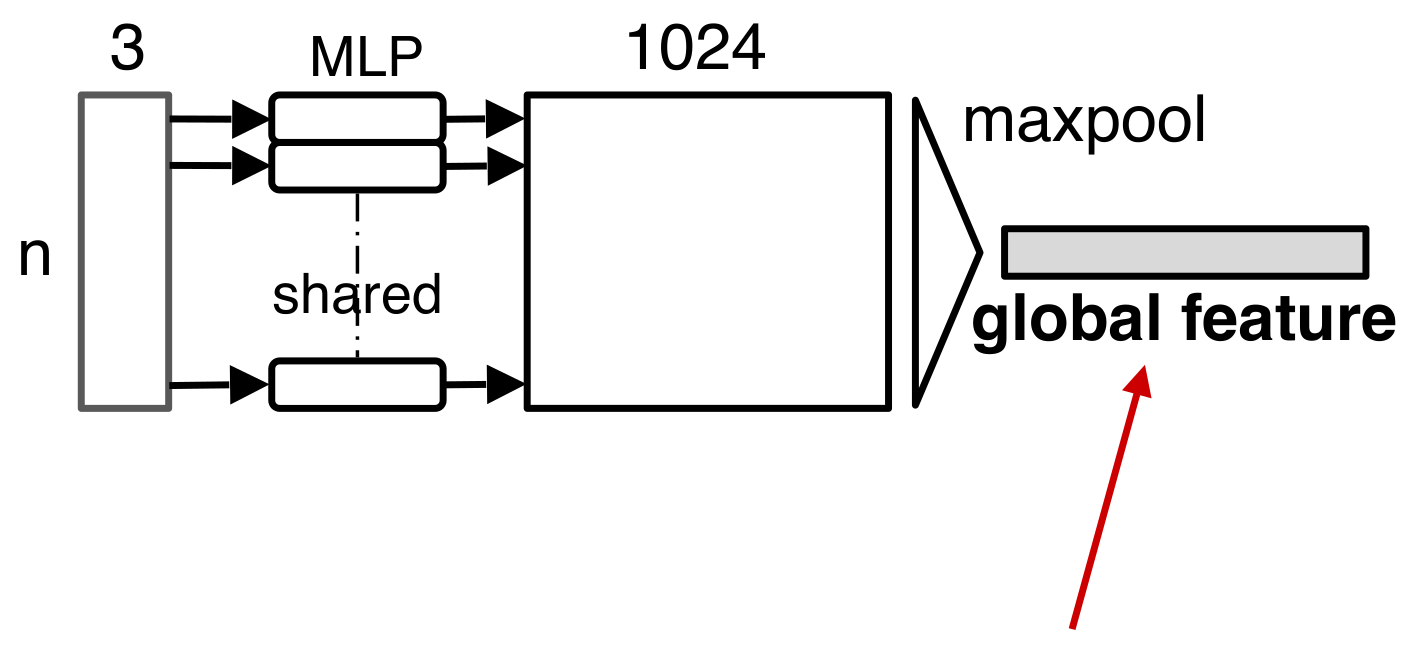
\includegraphics[width=0.55\textwidth]{sympool} \\
    Which points \underline{contribute} to the global feature vector? (\textbf{critical points}) \\
    Which additional points \underline{won't} affect the global feature vector? (\textbf{upper bound}) \\
    \blfootnote{Figure from CVPR presentation to \cite{qi2017pointnet}.}
    \pnote{
        Welche Punkte beeinflussen den Global Feature vektor? \\
        Welche kann man hinzufügen, ohne?
        \par
        Es sollte klar sein, dass nicht alle beitragen werden \\
        aufgrund von max pooling
    }
\end{frame}


\begin{frame}[c]{Visualizing Global Point Cloud Features}
    \centering
    \Large
    \begin{columns}
        \column{0.3\textwidth}
        \begin{itemize}
            \item Original Shape
                \vspace{2.5em}
            \item Critical Point Set
                \vspace{2.5em}
            \item Upper Bound Set
        \end{itemize}
        \column{0.6\textwidth}
        % trim=left bottom right top, clip
        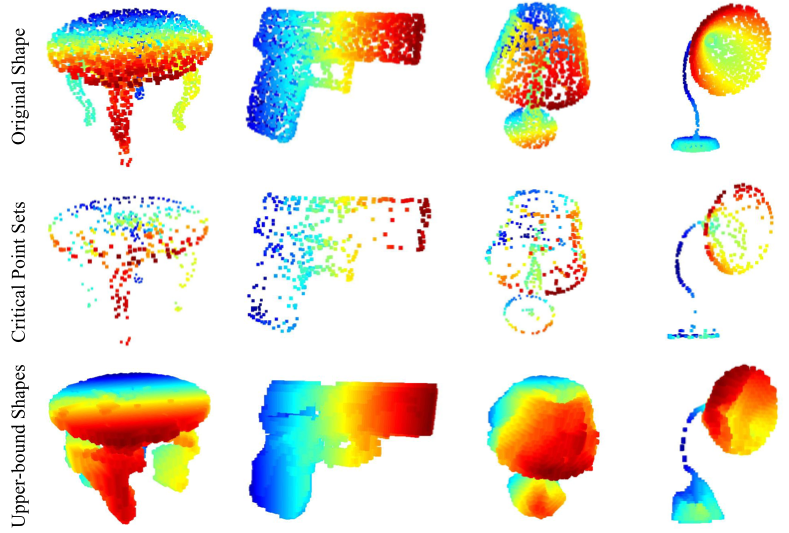
\includegraphics[height=0.7\textheight,trim=40 0 0 0,clip]{p56_68}
    \end{columns}
    \blfootnote{Figure from \cite{qi2017pointnet}.}
    \pnote{
        kritischen Punkte bilden ungefähr ursprüngliche Form \\
        Obere Schranke füllt zwischenräume
        \par
        Erinnerung an Robustheit ggü fehlenden Punkten
    }
\end{frame}


\begin{frame}[c]{Visualizing Global Point Cloud Features (OOS)}
    \centering
    \Large
    \begin{columns}
        \column{0.3\textwidth}
        \begin{itemize}
            \item Original Shape
                \vspace{2.5em}
            \item Critical Point Set
                \vspace{2.5em}
            \item Upper Bound Set
        \end{itemize}
        \column{0.6\textwidth}
        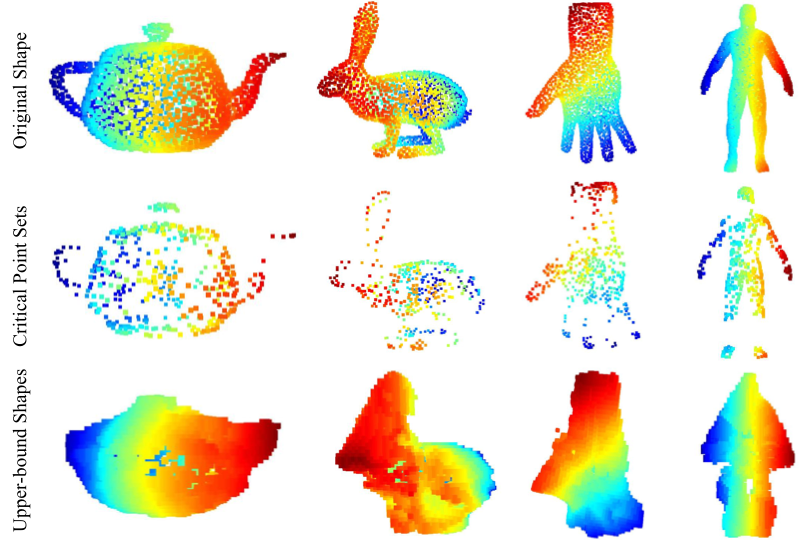
\includegraphics[height=0.7\textheight,trim=40 0 0 0,clip]{p57_69}
    \end{columns}
    \blfootnote{Figure from \cite{qi2017pointnet}.}
    \pnote{
        OOS = Out Of Specification \\
        Also nicht im Trainingsdatensatz enthaltene. \\
        Hier gehen teilweise dinge kaputt
        \par
        Erkenntnis: verallgemeinert gut
    }
\end{frame}


\begin{frame}[c]{Approach to Features Visualization}
    \centering
    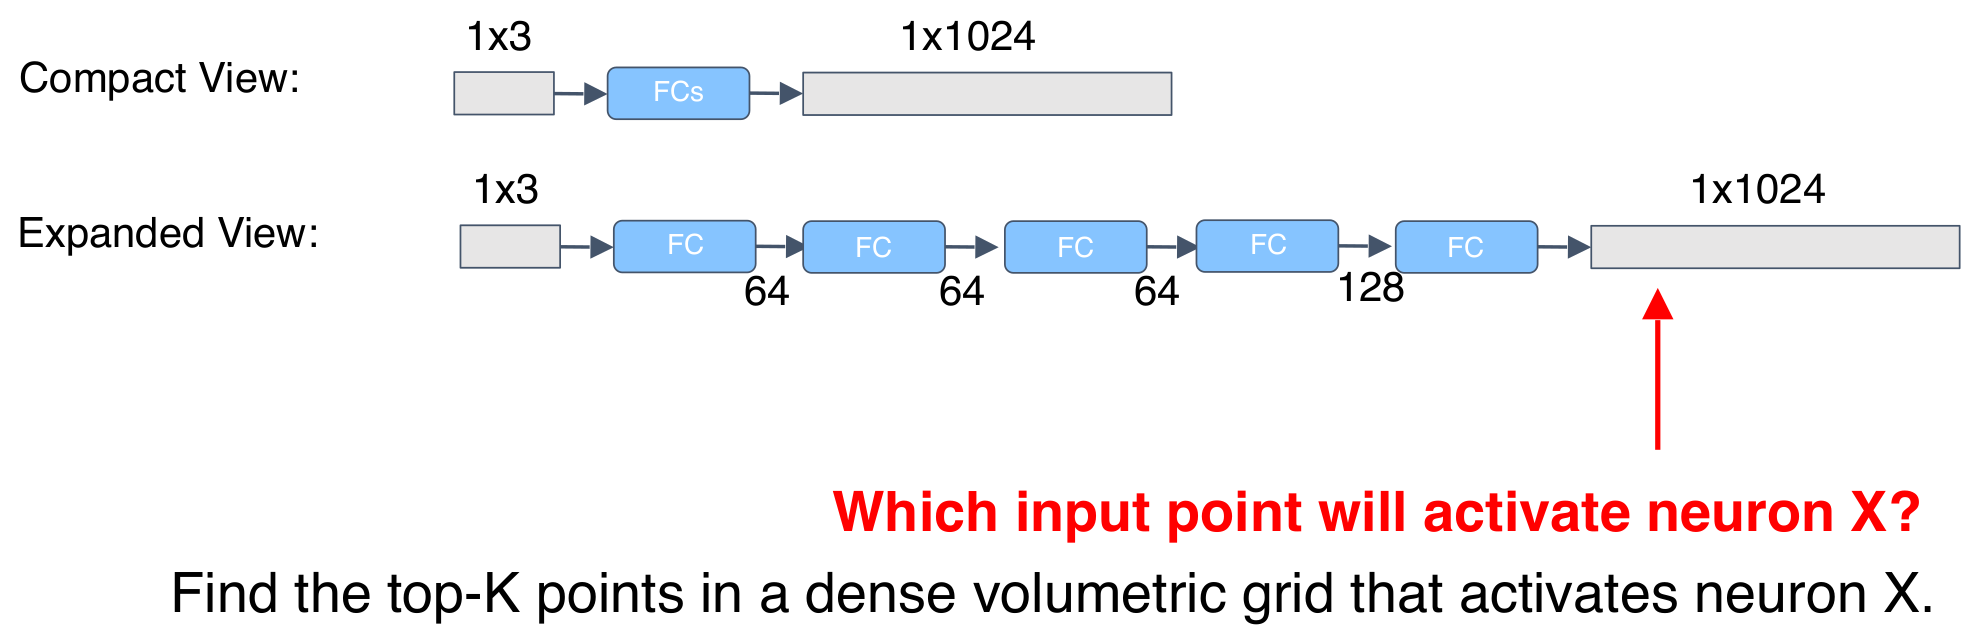
\includegraphics[width=\textwidth]{activation}
    \blfootnote{Figure from CVPR presentation to \cite{qi2017pointnet}.}
    \pnote{
        Visualisieren, was einzelne globale Features aktiviert
    }
\end{frame}


\begin{frame}[c]{Selective Visualization of Activation Features}
    \large
    \centering
    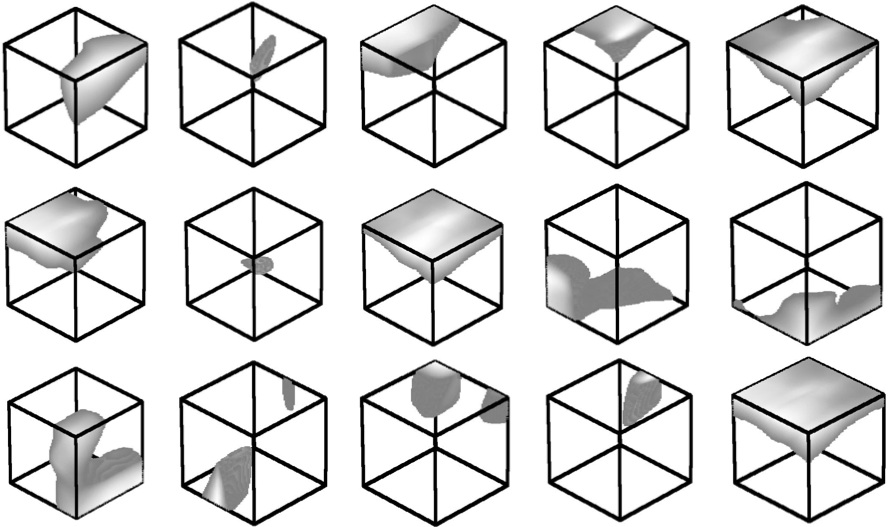
\includegraphics[height=0.7\textheight]{p68_80}
    \blfootnote{Figure from \cite{qi2017pointnet}.}
    \pnote{
        15 zufällig ausgewählte Features (der 1024) \\
        Man sieht, wie erwartet: räumliche Abdeckung
    }
\end{frame}
